%%% LaTeX Template: Two column article
%%%
%%% Source: http://www.howtotex.com/
%%% Feel free to distribute this template, but please keep to referal to http://www.howtotex.com/ here.
%%% Date: February 2011

%%% Preamble
\documentclass[	DIV=calc,%
							paper=a4,%
							fontsize=12pt,%
							onecolumn]{scrartcl}	 					% KOMA-article class

\usepackage{lipsum}													% Package to create dummy text
\usepackage[brazil]{babel}										% English language/hyphenation
\usepackage[protrusion=true,expansion=true]{microtype}				% Better typography
\usepackage{amsmath,amsfonts,amsthm}					% Math packages
\usepackage[pdftex]{graphicx}									% Enable pdflatex
\usepackage[svgnames]{xcolor}									% Enabling colors by their 'svgnames'
\usepackage[hang, small,labelfont=bf,up,textfont=it,up]{caption}	% Custom captions under/above floats
\usepackage{epstopdf}												% Converts .eps to .pdf
\usepackage{subfig}													% Subfigures
\usepackage{booktabs}												% Nicer tables
\usepackage{fix-cm}													% Custom fontsizes
\usepackage[utf8]{inputenc}
\usepackage[top=2.5cm, bottom=2.5cm, left=2.5cm, right=2.5cm]{geometry}
\usepackage[ddmmyyyy]{datetime}
\addto\captionsenglish{%
	\renewcommand\tablename{Tabela}
	\renewcommand\figurename{Figura}
} 
 

 
%%% Custom sectioning (sectsty package)
\usepackage{sectsty}													% Custom sectioning (see below)
\allsectionsfont{%															% Change font of al section commands
	\usefont{OT1}{phv}{b}{n}%										% bch-b-n: CharterBT-Bold font
	}

\sectionfont{%																% Change font of \section command
	\usefont{OT1}{phv}{b}{n}%										% bch-b-n: CharterBT-Bold font
	}



%%% Headers and footers
\usepackage{fancyhdr}												% Needed to define custom headers/footers
	\pagestyle{fancy}														% Enabling the custom headers/footers
\usepackage{lastpage}	

% Header (empty)
\lhead{}
\chead{}
\rhead{}
% Footer (you may change this to your own needs)

%% ====================================
%% ====================================
%% mude o rodape  do projeto
%% ====================================
%% ====================================

\lfoot{\footnotesize \texttt{Cabeamento estruturado} \textbullet ~Modelo de projeto}


\cfoot{}
\rfoot{\footnotesize página \thepage\ de \pageref{LastPage}}	% "Page 1 of 2"
\renewcommand{\headrulewidth}{0.0pt}
\renewcommand{\footrulewidth}{0.4pt}



%%% Creating an initial of the very first character of the content
\usepackage{lettrine}
\newcommand{\initial}[1]{%
     \lettrine[lines=3,lhang=0.3,nindent=0em]{
     				\color{DarkGoldenrod}
     				{\textsf{#1}}}{}}



%%% Title, author and date metadata
\usepackage{titling}															% For custom titles

\newcommand{\HorRule}{\color{DarkGoldenrod}%			% Creating a horizontal rule
									  	\rule{\linewidth}{1pt}%
										}

\pretitle{\vspace{-30pt} \begin{flushleft} \HorRule 
				\fontsize{50}{50} \usefont{OT1}{phv}{b}{n} \color{DarkRed} \selectfont 
				}

%% ====================================
%% ====================================
%% mude o titulo  do projeto
%% ====================================
%% ====================================

\title{Infraestrutura de Rede para Escritório e Armazém de Produtos}					% Title of your article goes here

%% ====================================



\posttitle{\par\end{flushleft}\vskip 0.5em}

\preauthor{\begin{flushleft}
					\large \lineskip 0.5em \usefont{OT1}{phv}{b}{sl} \color{DarkRed}}
\author{Carlos Alberto Zanella e Danilo Mendes Pusch}  	% Author name goes here


\postauthor{\footnotesize \usefont{OT1}{phv}{m}{sl} \color{Black} 
					\\Universidade Tecnológica Federal do Paraná - Câmpus Cornélio Procópio 								% Institution of author
					\par\end{flushleft}\HorRule}

\date{}																				% No date




%%% Begin document
\begin{document}
\maketitle
\thispagestyle{fancy} 	
\thispagestyle{empty}		% Enabling the custom headers/footers for the first page 
% The first character should be within \initial{}




%% ====================================
%% ====================================
%% mude o resumo  do projeto
%% ====================================
%% ====================================

\initial{E}\textbf{ste projeto irá prover uma infraestrutura de rede de dados para atender a demanda necessária de rede cabeada para um escritório administrativo e um armazém de produtos. As premissas deste projeto são uma rede cabeada projetada de alta velocidade (até 10 Gigabit), onde cada ponto de rede permita a instalação de no mínimo 2 dispositivos de rede por local de trabalho (por exemplo computador e telefone). Deverá contemplar também pontos de rede no escritório para a instalação de dispositivos de rede sem fio. Entre as etapas desse projeto estão contemplados o levantamento da planta física, elaboração da planta lógica, memorial descritivo dos equipamentos passivos de rede, o levantamento da quantidade / custos, o plano de certificação e o orçamento.  \ref{fig4}.}


%% ====================================
\begin{figure}
	\centering
	
\includegraphics{utfpr}
\end{figure}

\vspace{2cm}
\centerline{\textit{\textbf{\today}}}

\clearpage
    \renewcommand*\listfigurename{Lista de figuras}
\listoffigures

\renewcommand*\listtablename{Lista de tabelas}
\listoftables




\clearpage
\renewcommand{\contentsname}{Sumário}
\tableofcontents
\clearpage

%% ====================================
%% ====================================
%% Inicio do texto
%% ====================================
%% ====================================
\section{Introdução}
Este projeto visa implementar infraestrutura de rede com cabeamento estruturado para um novo escritório administrativo e um novo armazém de produtos na Gerência de Manutenção Operacional de uma grande cooperativa agroindustrial. Apesar do projeto ser real, a identidade e o porte do cliente serão omitidos por motivo de confidencialidade. 

\subsection{Benefícios}
A implementação desse projeto deve trazer como benefícios primeiramente facilitar o gerenciamento e garantir a segurança da rede tanto para o escritório administrativo como para o armazém de insumos. Além disso deve contemplar a possibilidade de uma possível expansão futura e atender a requisitos baseados em normas técnicas, além de fornecer a performance necessária para a execução de todas as aplicações.

\subsection{Organizações Envolvidas}
Este projeto, apesar de ser real, por motivo de confidencialidade não identificaremos a organização envolvida. Todo projeto será executado por equipe própria, não envolvendo outras empresas na execução, somente na aquisição de equipamentos. Os perfis de funcionários envolvidos são:
\begin{itemize}
	\item Analista de compras: realizar cotação e compra dos equipamentos. 
	\item Analista financeiro: responsável pela aprovação financeira e pagamentos.
	\item Engenheiro elétrico: realiza o acompanhamento das instalações elétricas necessárias. 
	\item Desenhista: realiza as plantas físicas e lógicas do projeto. 
	\item Instalador: responsável por realizar a instalação dos passivos de rede conforme projeto. 
	\item Analista de TI: acompanha e ativa a conectividade de acesso a rede da empresa. 
	\item Empresa de telecom: instala os troncos de telefonia.  
\end{itemize}


\section{Estado atual}
Como os ambientes em que o projeto será implementado são novos e acabam de ser construídos, o estado atual da rede não se aplica a essa situação. 

\section{Requisitos}
Provisionar uma rede cabeada projetada de alta velocidade (até 10 Gigabit). Permitir a instalação de no mínimo 2 dispositivos de rede por local de trabalho (telefone IP / micro ou Thin Client). Pontos de rede adicionais para instalação de dispositivos sem fio (Wi-Fi) e também para possível expansão posterior. 

\section{Usuários e Aplicativos}
Este ambiente deverá comportar uma central de distribuição da empresa. A principio a quantidade de usuários nesse setor deverá ser a que consta na relação abaixo, sem uma previsão inicial de expansão. O projeto deve permitir a instalação de equipamentos para rede sem-fio (Wi-Fi) com pontos de rede já devidamente previstos e instalados. 


\subsection{Usuários}
A central de distribuição deverá contar com a seguinte equipe:
\begin{itemize}
	\item 6 auxiliares administrativos
	\item 2 faturistas
	\item 1 secretária
	\item 4 estoquistas
	\item 2 analistas de RH
	\item 1 chefe de departamento
		
\end{itemize}

\subsection{Aplicativos}
Relação dos aplicativos e seus níveis críticos de uso.
\begin{itemize}
	\item ERP (Uniface): criticidade alta. 
	\item Sistema de gestão de ativos (IBM Maximo): criticidade média.
	\item Sistema dos coletores: criticidade média. 
	\item Arterisk telefonia IP: criticidade alta. 
	\item Sistema operacional Windows: criticidade média.  
	\item Pacote Office: criticidade média. 
\end{itemize}


\section{Estrutura predial existente}
Estrutura predial existente conforme figura \ref{figura1}. 
\begin{figure}
	\centering
	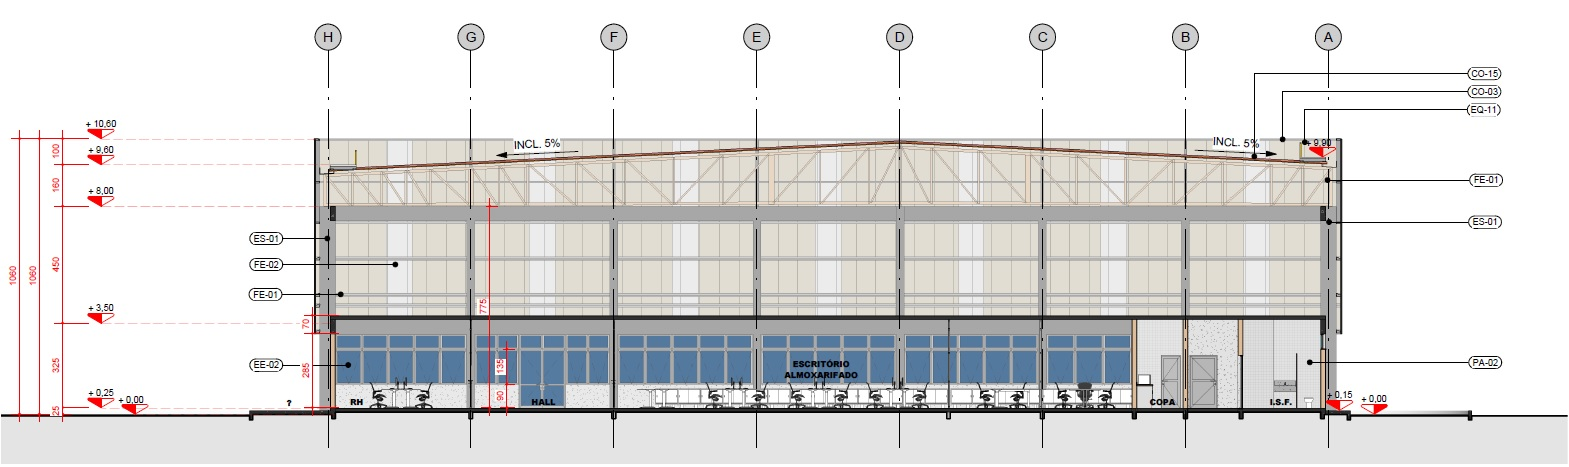
\includegraphics[width=\textwidth]{figura1}
	\caption{Estrutura predial existente}
	\label{figura1}
\end{figure}

\section{Planta Lógica - Elementos estruturados}

\subsection{Estado atual}
Planta baixa e situação atual do prédio conforme figura \ref{figura2}. 
\begin{figure}
	\centering
	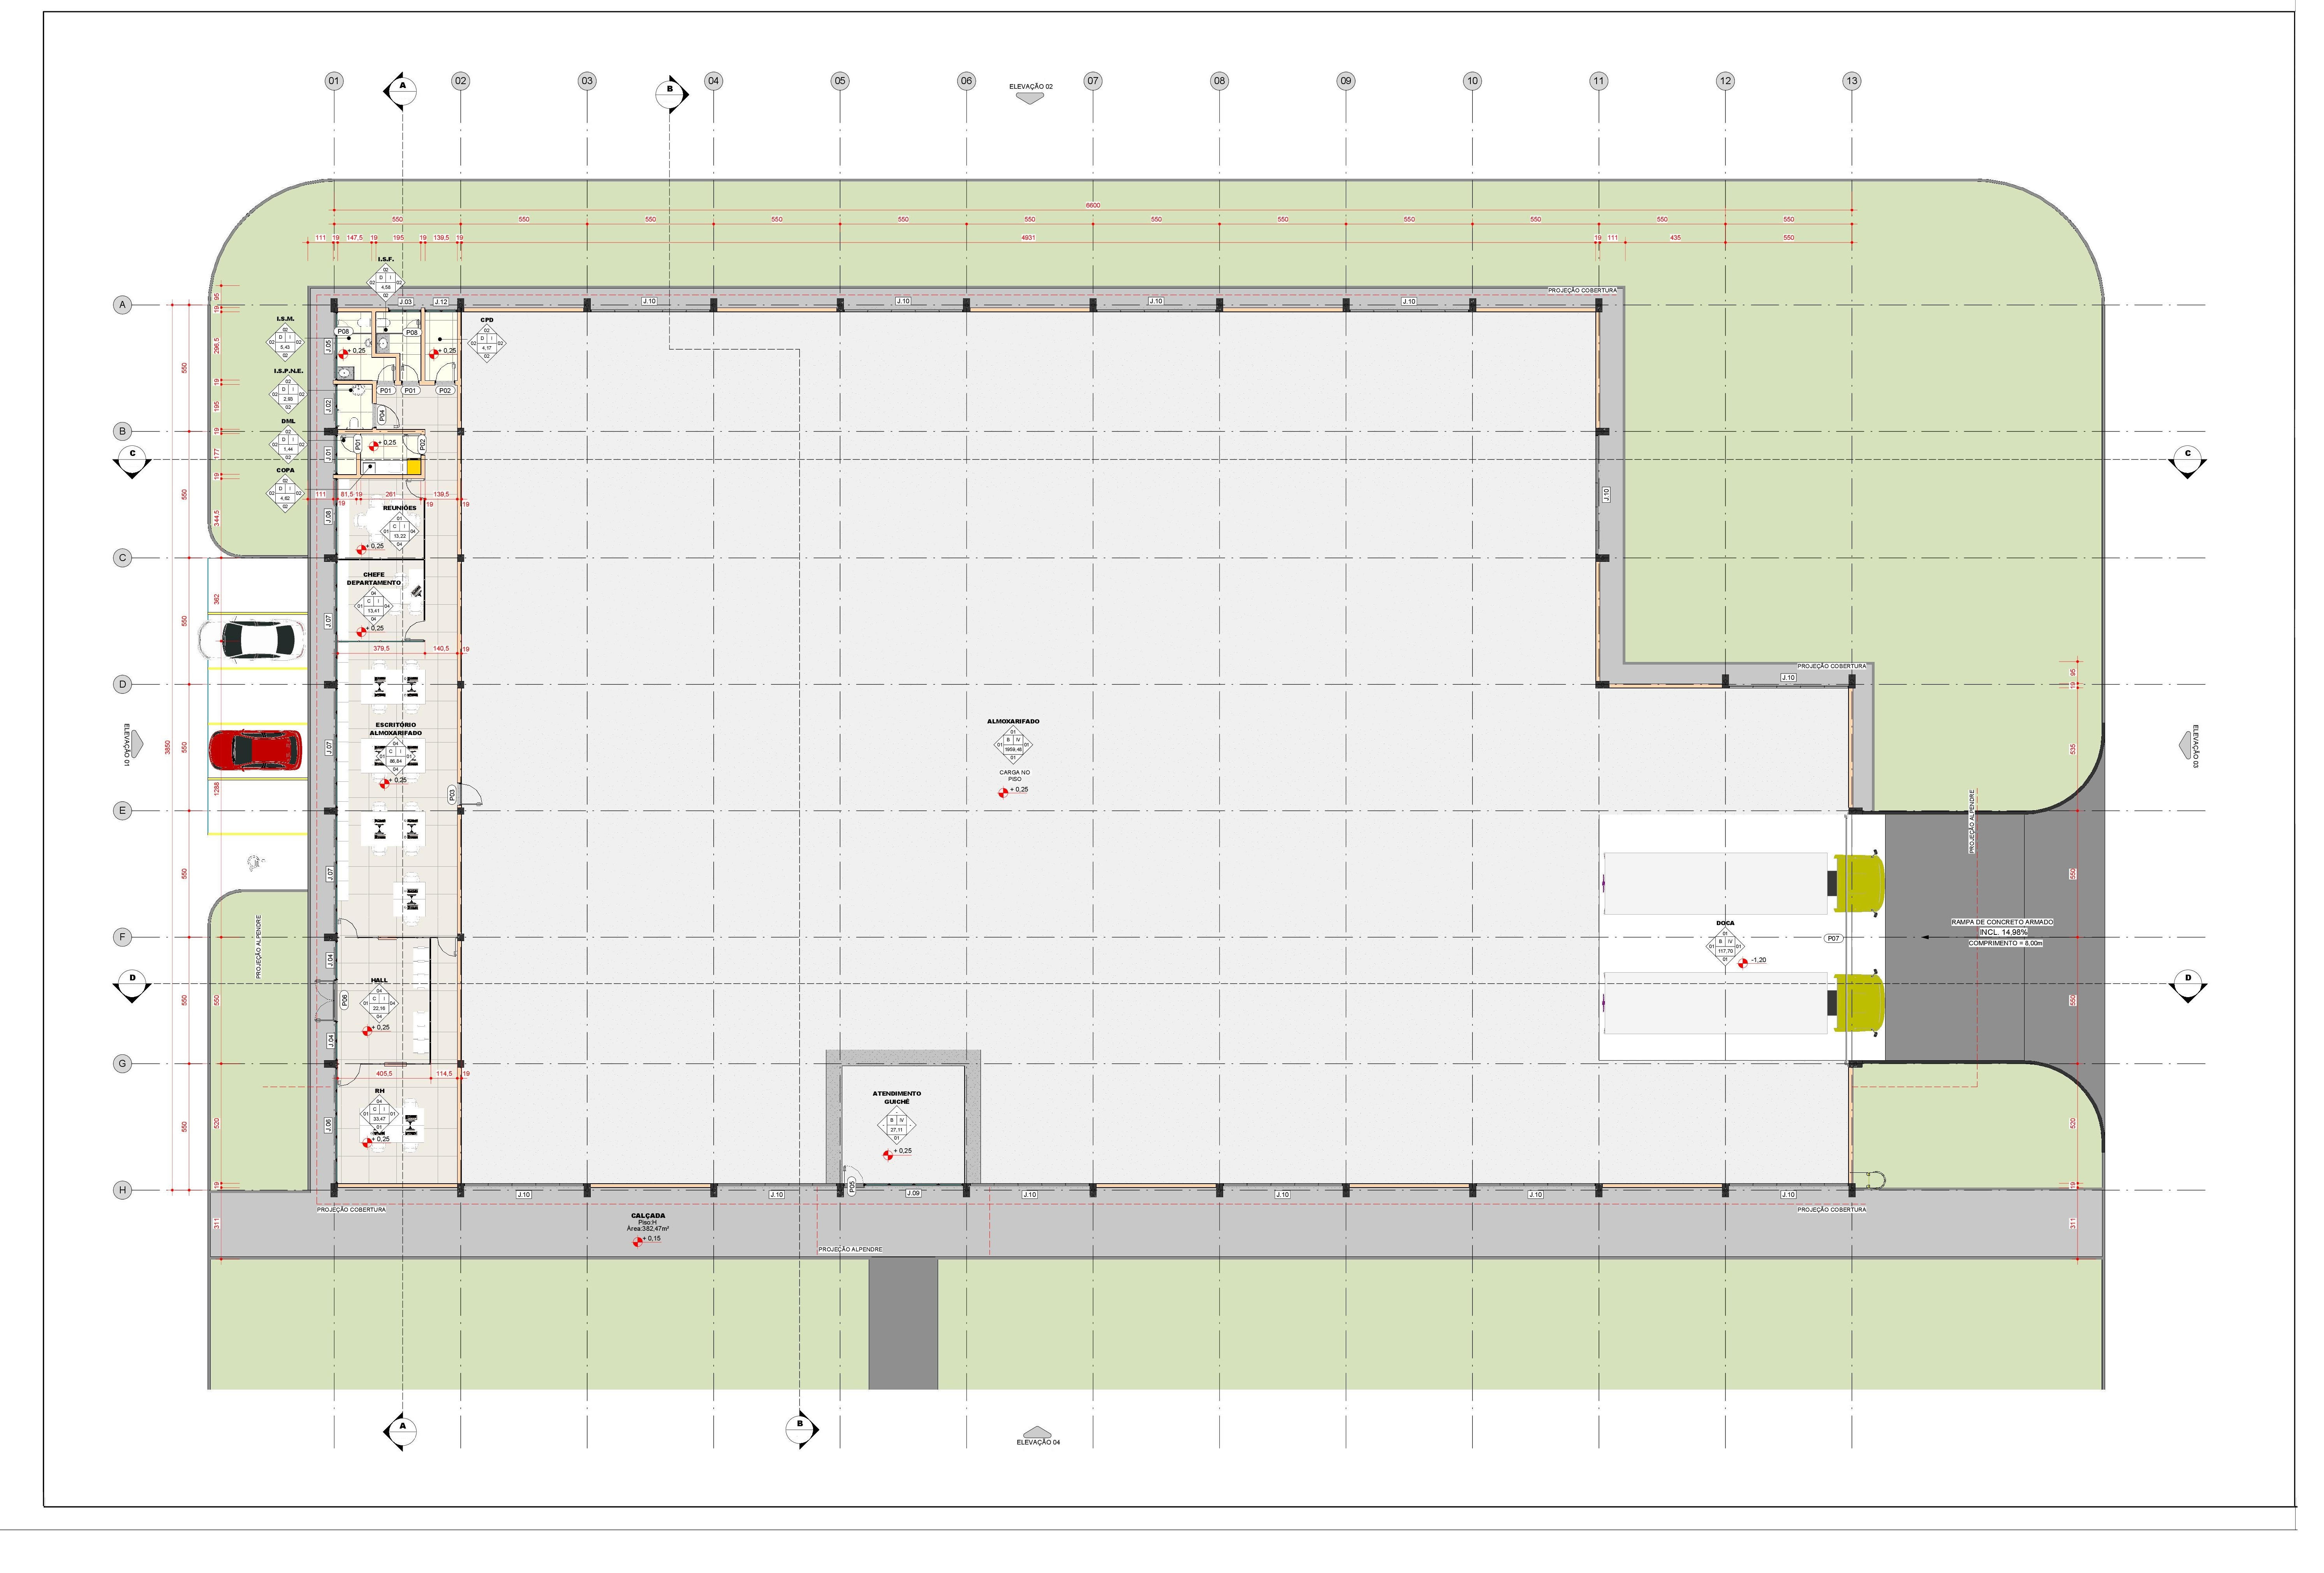
\includegraphics[width=\textwidth]{figura2}
	\caption{Planta baixa}
	\label{figura2}
\end{figure}

\subsection{Topologia}
De acordo com Augusto \cite{ID1}, a topologia pode ser entendida como a maneira pela qual os enlaces de comunicação e dispositivos de comutação estão interligados, provendo efetivamente a transmissão do sinal entre nós da rede. [...] Podemos dizer que a topologia física de uma rede local compreende os enlaces físicos de ligação dos elementos computacionais da rede, enquanto a topologia lógica da rede se refere à forma através da qual o sinal é efetivamente transmitido entre um computador e outro. Planta lógica conforme figura \ref{figura3}. 
\begin{figure}
	\centering
	\includegraphics[width=\textwidth]{figura3}
	\caption{Planta lógica}
	\label{figura3}
\end{figure}

Podemos ver também os modelos de rack que serão utilizados abaixo na tabela \ref{tab1}.

\begin{table}[h!]
\centering
\caption{Exemplo de racks utilizados}
\label{tab1}
\begin{tabular}{|l|l|l|}
\hline
\multicolumn{3}{|l|}{Racks utilizados} \\ \hline
1        & Rack 12U          & 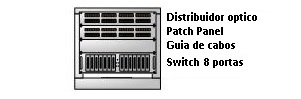
\includegraphics[scale=0.8]{figura5}        \\ \hline
2        & Rack 40U        & 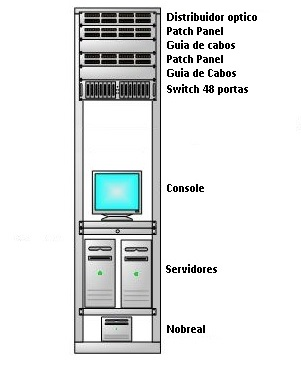
\includegraphics[scale=0.8]{figura6}        \\ \hline
\end{tabular}
\end{table}

\subsection{Encaminhamento}
Relação do encaminhamento e seus respectivos custos conforme figura \ref{figura4}.  
\begin{figure}
	\centering
	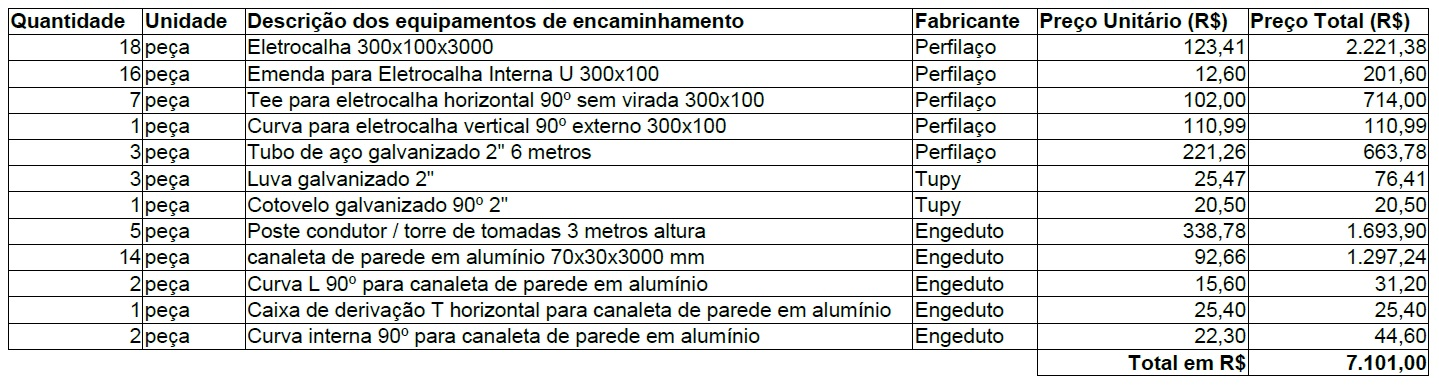
\includegraphics[width=\textwidth]{figura4}
	\caption{Encaminhamento e custos}
	\label{figura4}
\end{figure}

\subsection{Memorial descritivo}

Relacione todos os equipamentos passivos que serão utilizados, tipo, fabricante, quantidade.

\subsection{Identificação dos cabos}
A identificação dos cabos será realizada de acordo com a norma NBR 14565:2000. A relação de todos os passivos utilizados, inclusive os cabos, bem como os custos envolvidos consta no item 6.4, memorial descritivo deste documento. 

\section{Implantação}
Estabeleça um cronograma de implantação:
Remoção de equipamentos existentes (destino para descarte), instalação dos condutores, instalação dos cabos, 
identificação dos cabos, montagem dos racks, certificação, etc... Crie atividades e estabeleça o tempo de execução. Se for um projeto real, indique também quais os responsáveis pela execução do projeto e de cada uma das etapas.

Defina marcas (e padrões) e fornecedores se for o caso. Atenção a contratados e subcontratados para a realização das atividades. Estabeleça a responsabilidade de execução da atividade e também da validação dela.

Utilize algum software para gerear o cronograma. Excel,etc. O fundamental é dividir em etapas, descrever e estimar o tempo de cada uma delas.

Segue uma relação de ferramentas:
http://asana.com/, 
https://trello.com/, 
http://www.ganttproject.biz/, 
http://www.orangescrum.org/. 

\section{Plano de certificação}
Quais seriam as etapas para a certificação? 
Quais os locais e horários para execução da certificação na rede? Toda rede será certificada?
Como os testes seriam executados?
Quais relatórios de certificação serão (ou deveriam ser) entregues? 

\section{Plano de manutenção}

A manutenção desta rede deverá seguir as melhores práticas e deverá ser registrada no sistema de gestão de Ativos IBM Maximo de acordo com os seguintes critérios: 
\begin{itemize}
	\item Manutenção Preventiva: Realizada mensalmente na Central de Distribuição pelos técnicos do setor de manutenção de informática, subordinado ao departamento de infraestrutura e suporte de TI. Será executado um plano de trabalho onde é realizada a verificação das conexões e a checagem visual do estado geral dos equipamentos, e também a execução da limpeza adequada. 
	\item Manutenção Corretiva (interna): Realizada pelos analistas departamento de infraestrutura e suporte de TI. Consiste na solução dos problemas detectados na manutenção preventiva ou pela abertura de incidentes no sistema de Service Desk.
	\item Manutenção Corretiva (terceiros): Realizada por empresa de suporte externa. Consiste na solução dos problemas detectados na manutenção preventiva ou corretiva não solucionados internamente ou quando envolvem garantias de equipamentos. Consiste na manutenção e/ou troca de componentes. As manutenções corretivas por terceiros são realizadas por empresas contratadas pelo departamento de compras da empresa, negociadas pelo departamento de gestão de TI e com aprovação técnica do departamento de infraestrutura e suporte de TI.
\end{itemize}

\subsection{Plano de expansão}
A expansão da infraestrutura de tecnologia da central de distribuição deverá ser aprovada pela superintendência administrativa da empresa. Posteriormente, serão definidas as configurações de hardwares e softwares necessárias pelo departamento de infraestrutura e suporte de TI, bem como o projeto de implantação deve ser definido pelo setor de gestão de projetos, subordinado ao departamento de gestão de TI. Poderá ser executado por equipe interna do setor de manutenção de TI ou por empresa contratada. 

\section{Risco}
Enumerar e explicar os riscos do projeto.

\section{Orçamento}
Crie uma relação de orçamentos baseado na seções anteriores.

\section{Recomendações}
Observações e recomendações para o cliente.

\section{Referências bibliográficas}
Utilize o mendley, o jabref ou diretamente o bibtex para gerenciar suas referências biliográficas. As referências são criadas automaticamente de acordo com o uso no texto.

Exemplo: Redes de computadores, segundo \cite{t2013} é considerada..... Já \cite{kurose2010} apresenta uma versão...

Analisando os pressupostos de \cite{ref3} e \cite{ref4} concluimos que....


\renewcommand\refname{} %%Referências bibliográficas}  
\bibliographystyle{ieeetr}
\bibliography{referencias}  












%% ***********************************************************************
%% === remover daqui =====================================================
%% ***********************************************************************
=================================================
\section{Elementos textuais - Alguns exemplos}

Esta seção apresenta exemplos de elementos textuais. \textbf{Remova-a da versão final do texto}.


\subsection{Colocar elementos em itens}

Texto antes da lista

\begin{itemize}
	\item First item in a list 
	\item Second item in a list 
	\item Third item in a list
\end{itemize}

\subsubsection{Uma subseção de terceiro nivel}

Exemplo de uma subseção

\subsection{Tabelas}

Utilize o site http://www.tablesgenerator.com/ para elaborar as tabelas de seu trabalho.
Para adicionar uma tabela utilize: a tag input, passando o arquivo da tabela como parametro

\begin{table}[h!] % coloque h! para forcar a posicao
\centering
\caption{Modifique a legenda e crie um label}
\label{tab2} %com este label vc faz referencia no texto
\begin{tabular}{|l|l|l|l|l|}
\hline
\multicolumn{1}{|c|}{\textbf{Este é um exemplo de tabela}} & \multicolumn{2}{c|}{\textbf{C1}} & \multicolumn{2}{c|}{\textbf{C2}} \\ \hline
Você pode criar a tabela no excel                          & 1              & 2               & 3               & 4              \\ \hline
Exportar para CSV                                          & 5              & 6               & 7               & 8              \\ \hline
E importar no Table Generator                              & 9              & 10              &                 &                \\ \hline
\multicolumn{5}{|c|}{\textit{Gere o tex, e adicione em seu arquivo}}                                                             \\ \hline
\end{tabular}
\end{table}

Dentro do arquivo você deve definir o label e pode utilizá-lo para referenciar. Exemplo:
Na tab \ref{tab2} temos a relação de ....


Você também pode modificar a tabela manualmente, incluindo, por exemplo h! dentro de sua definição. Veja no exemplo tab2.tex

\subsection{Figuras}

As figuras podem ser no formato PDF, JPG, PNG. Você pode referenciá-las da mesma maneira que tabelas. Exemplo: A figura \ref{fig1} apresenta.....

Não se preocupe o local em que a figura será renderizada em seu texto. Preocupe-se em criar referência para ela, ou seja, toda figura e tabela deve conter pelo menos uma referência no texto.

\begin{figure}
\centering
\includegraphics[width=\textwidth]{fig1}
\caption{Esquema lógico}
\label{fig1}
\end{figure}


\begin{figure}
	\centering
	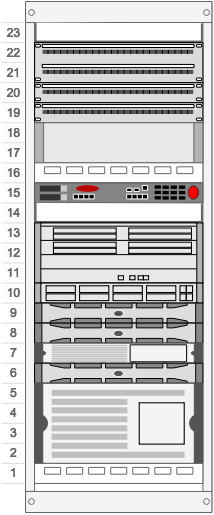
\includegraphics[]{fig2}
	\caption{Exemplo de figura sem escala}
	\label{fig2}
\end{figure}

Você pode rotacionar figuras também. Para isso utilize o parâmetro angle=-90. Repare que a escala da figura foi modificada pelo parametro height. Você também pode utilizar scale

\begin{figure}
	\centering
	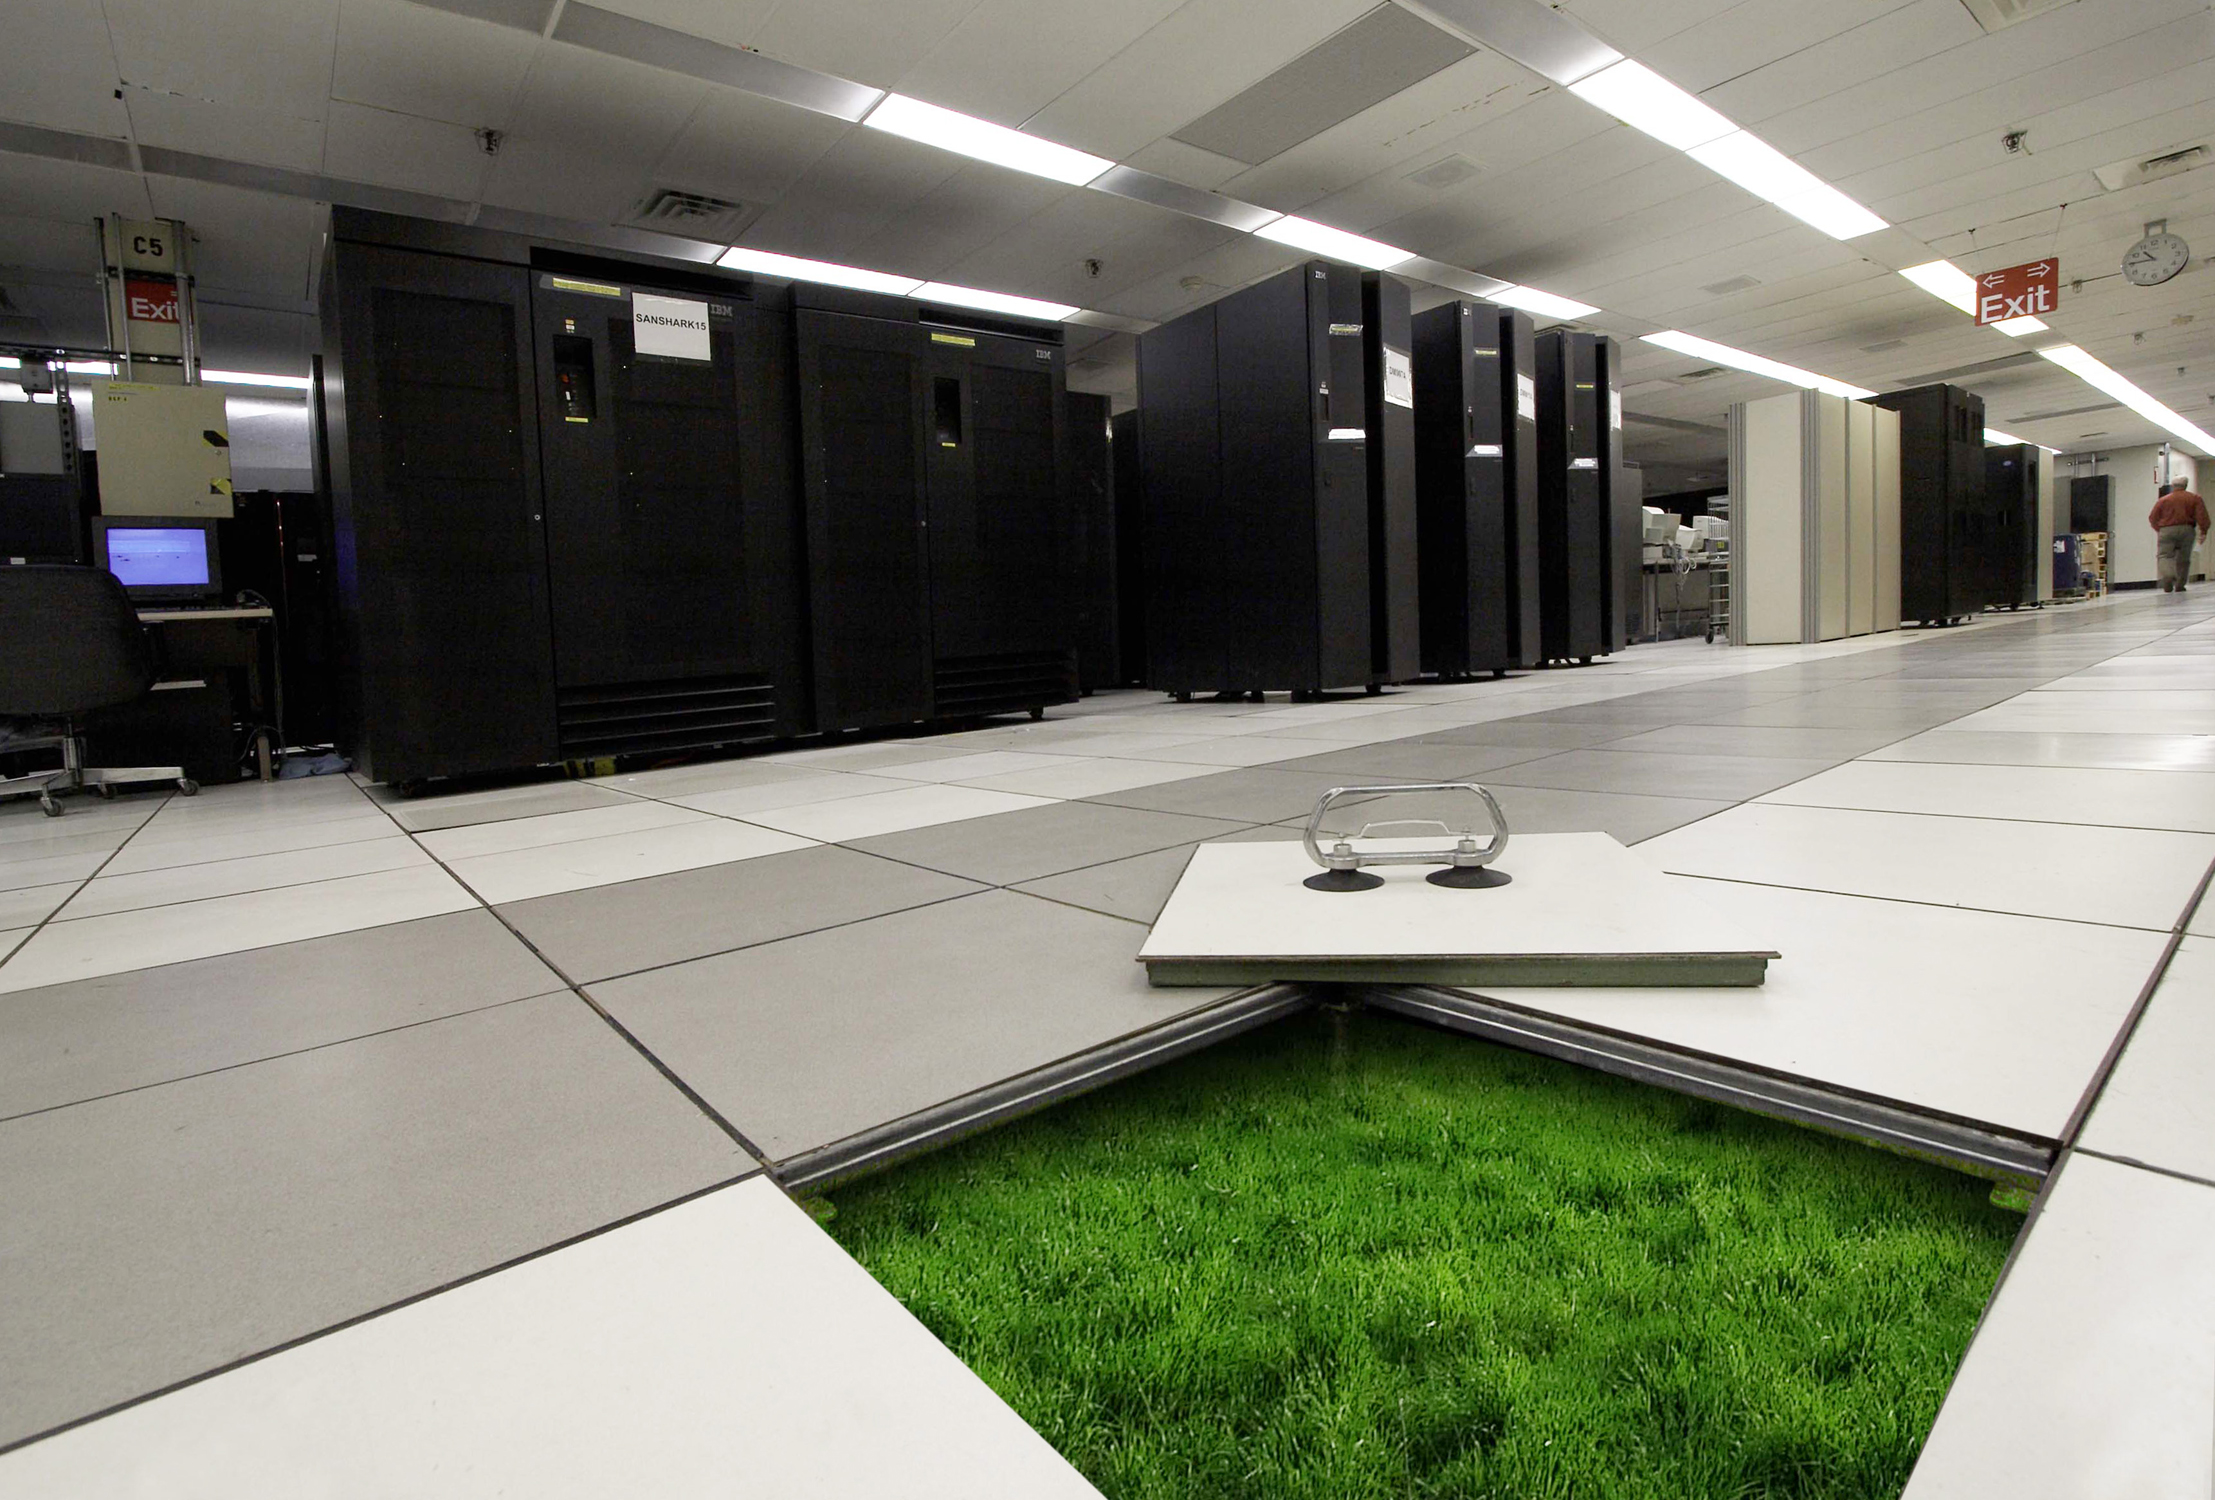
\includegraphics[height=\textwidth,angle=-90]{fig3}
	\caption{Exemplo de figura rotacionada}
	\label{fig3}
\end{figure}

Você também pode inserir páginas de outro tamanho em seu texto. Isto irá ajudar a inserir imagens maiores, como as desenvolvidas em CAD. Segue um exemplo na figura \ref{fig4} e figura \ref{fig5}.


%inicio dos comandos para criar uma nova pagina A3
\clearpage
\KOMAoptions{paper=a3, pagesize}
\recalctypearea

\begin{figure}
	\centering
	\makebox[\textwidth][c]{
		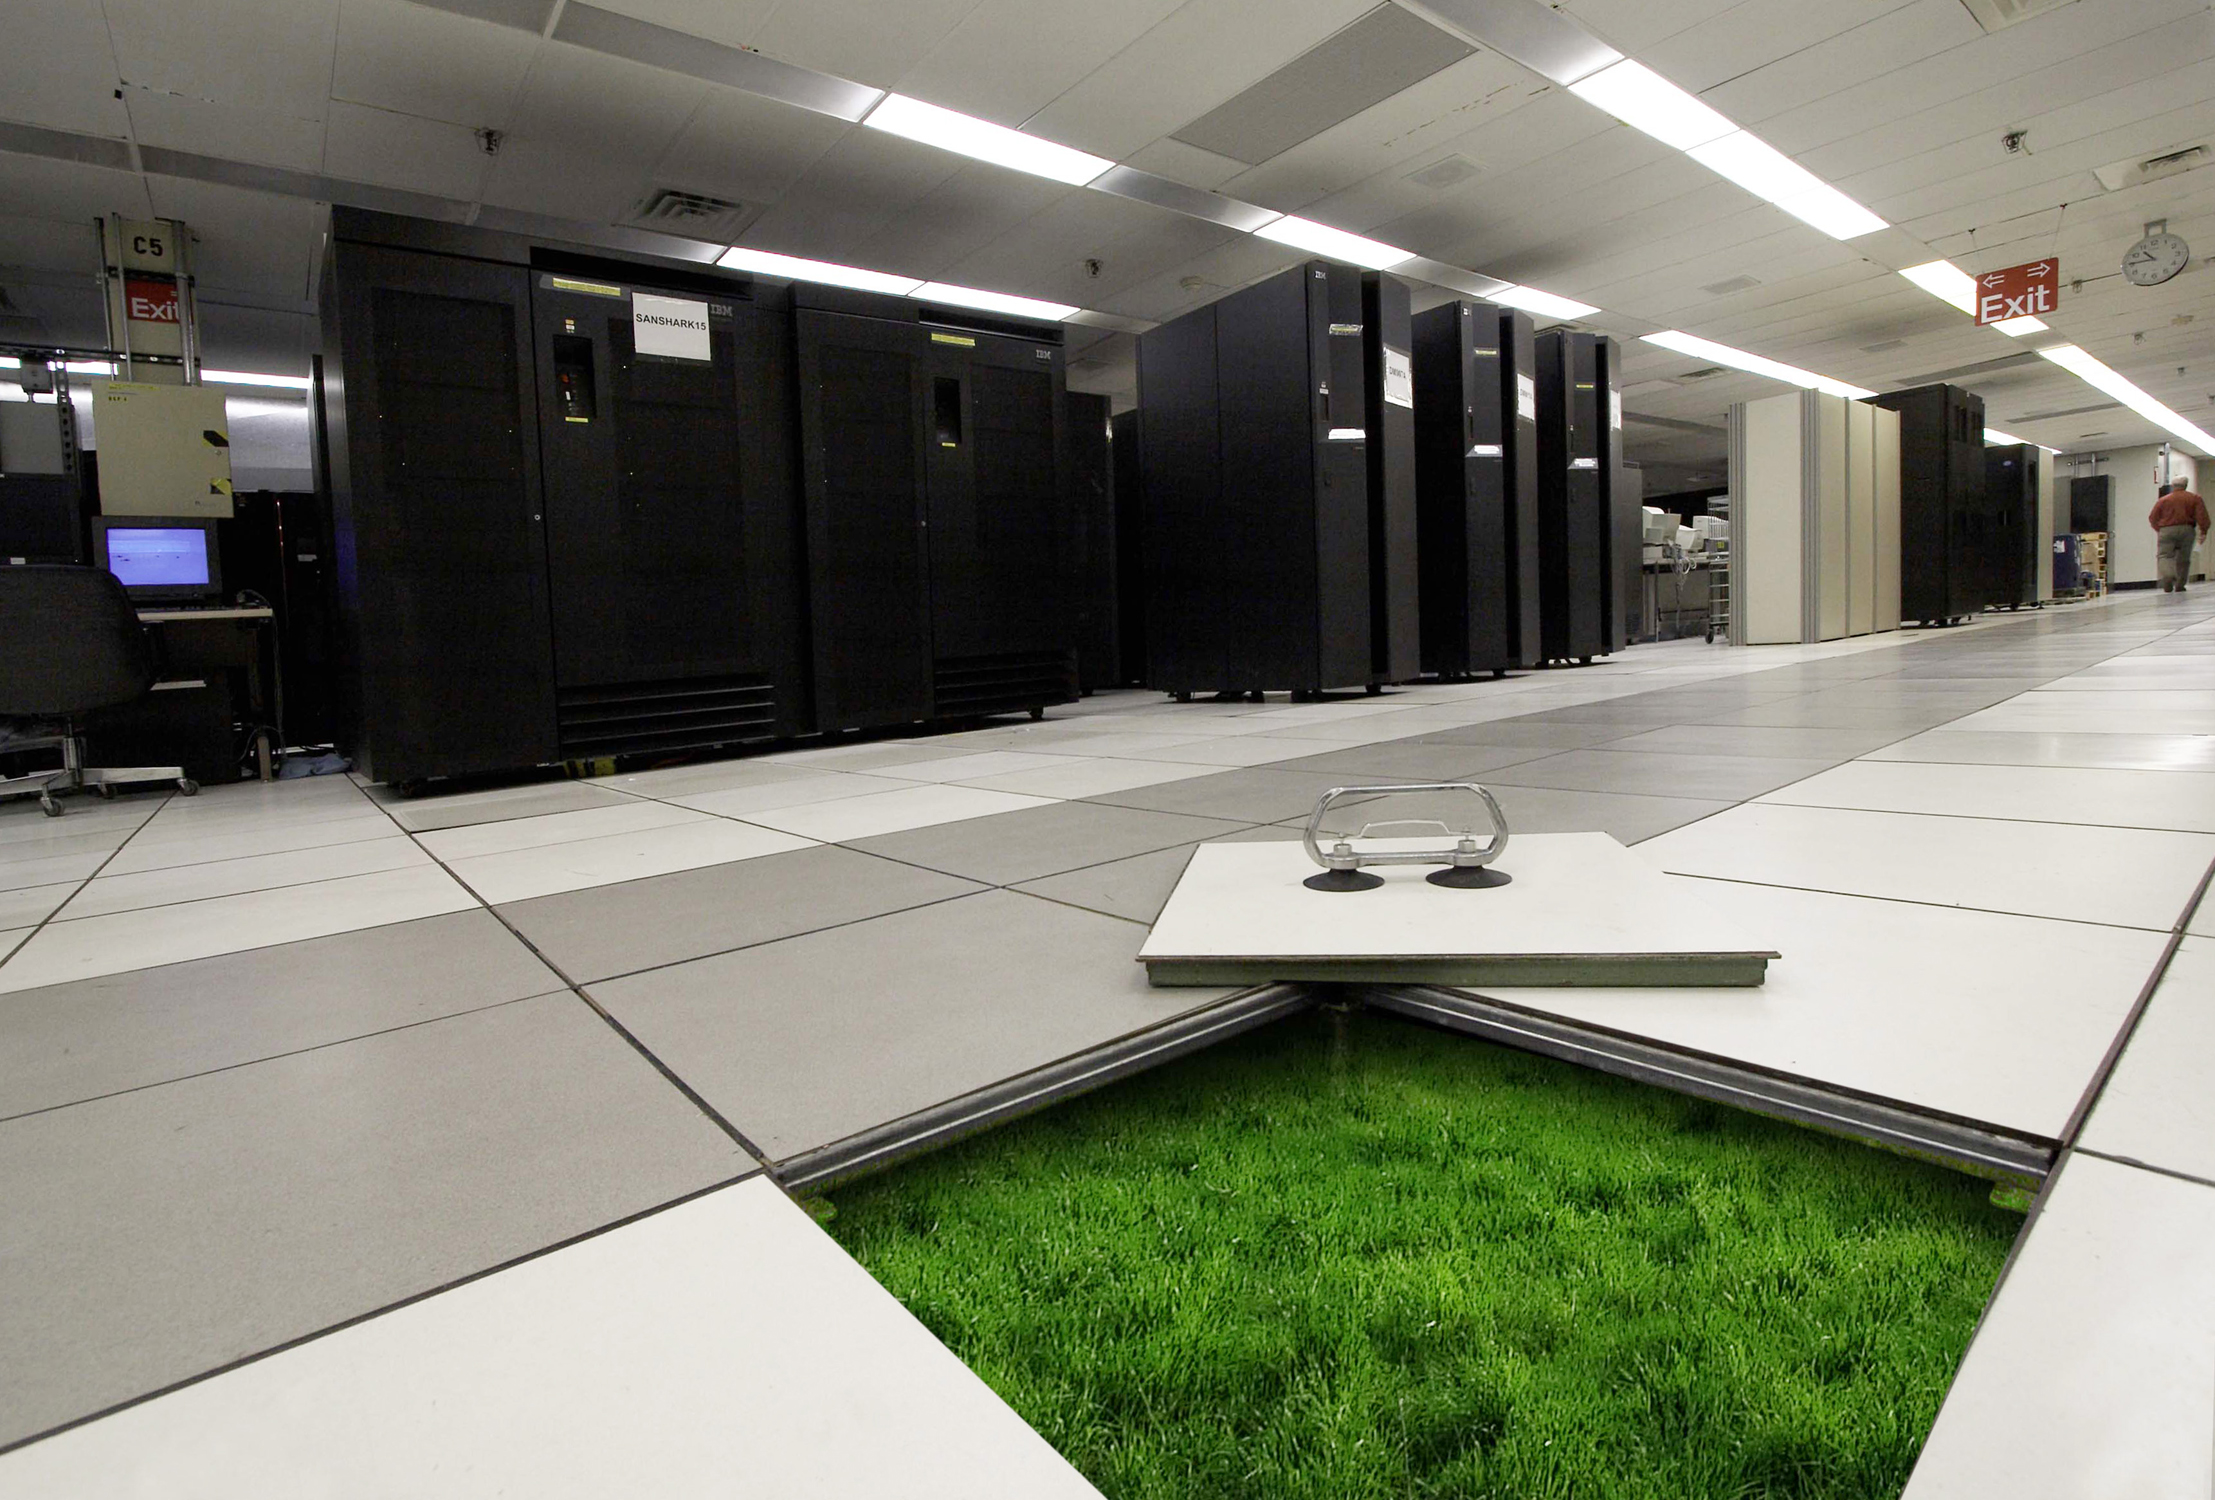
\includegraphics[height=\textheight]{fig3}}
	\caption{Exemplo de figura inserida em uma página A3}
	\label{fig4}
\end{figure}

%Retornar ao formato A4
\clearpage
\KOMAoptions{paper=a4, pagesize}
\recalctypearea
%-- reinicio em A4 


%inicio dos comandos para criar uma nova pagina A3 horizontal
\clearpage
\KOMAoptions{paper=a3, paper=landscape, DIV=20}
\recalctypearea

	
\begin{figure}
%	\centering
	\noindent\makebox[\textwidth][c]{
		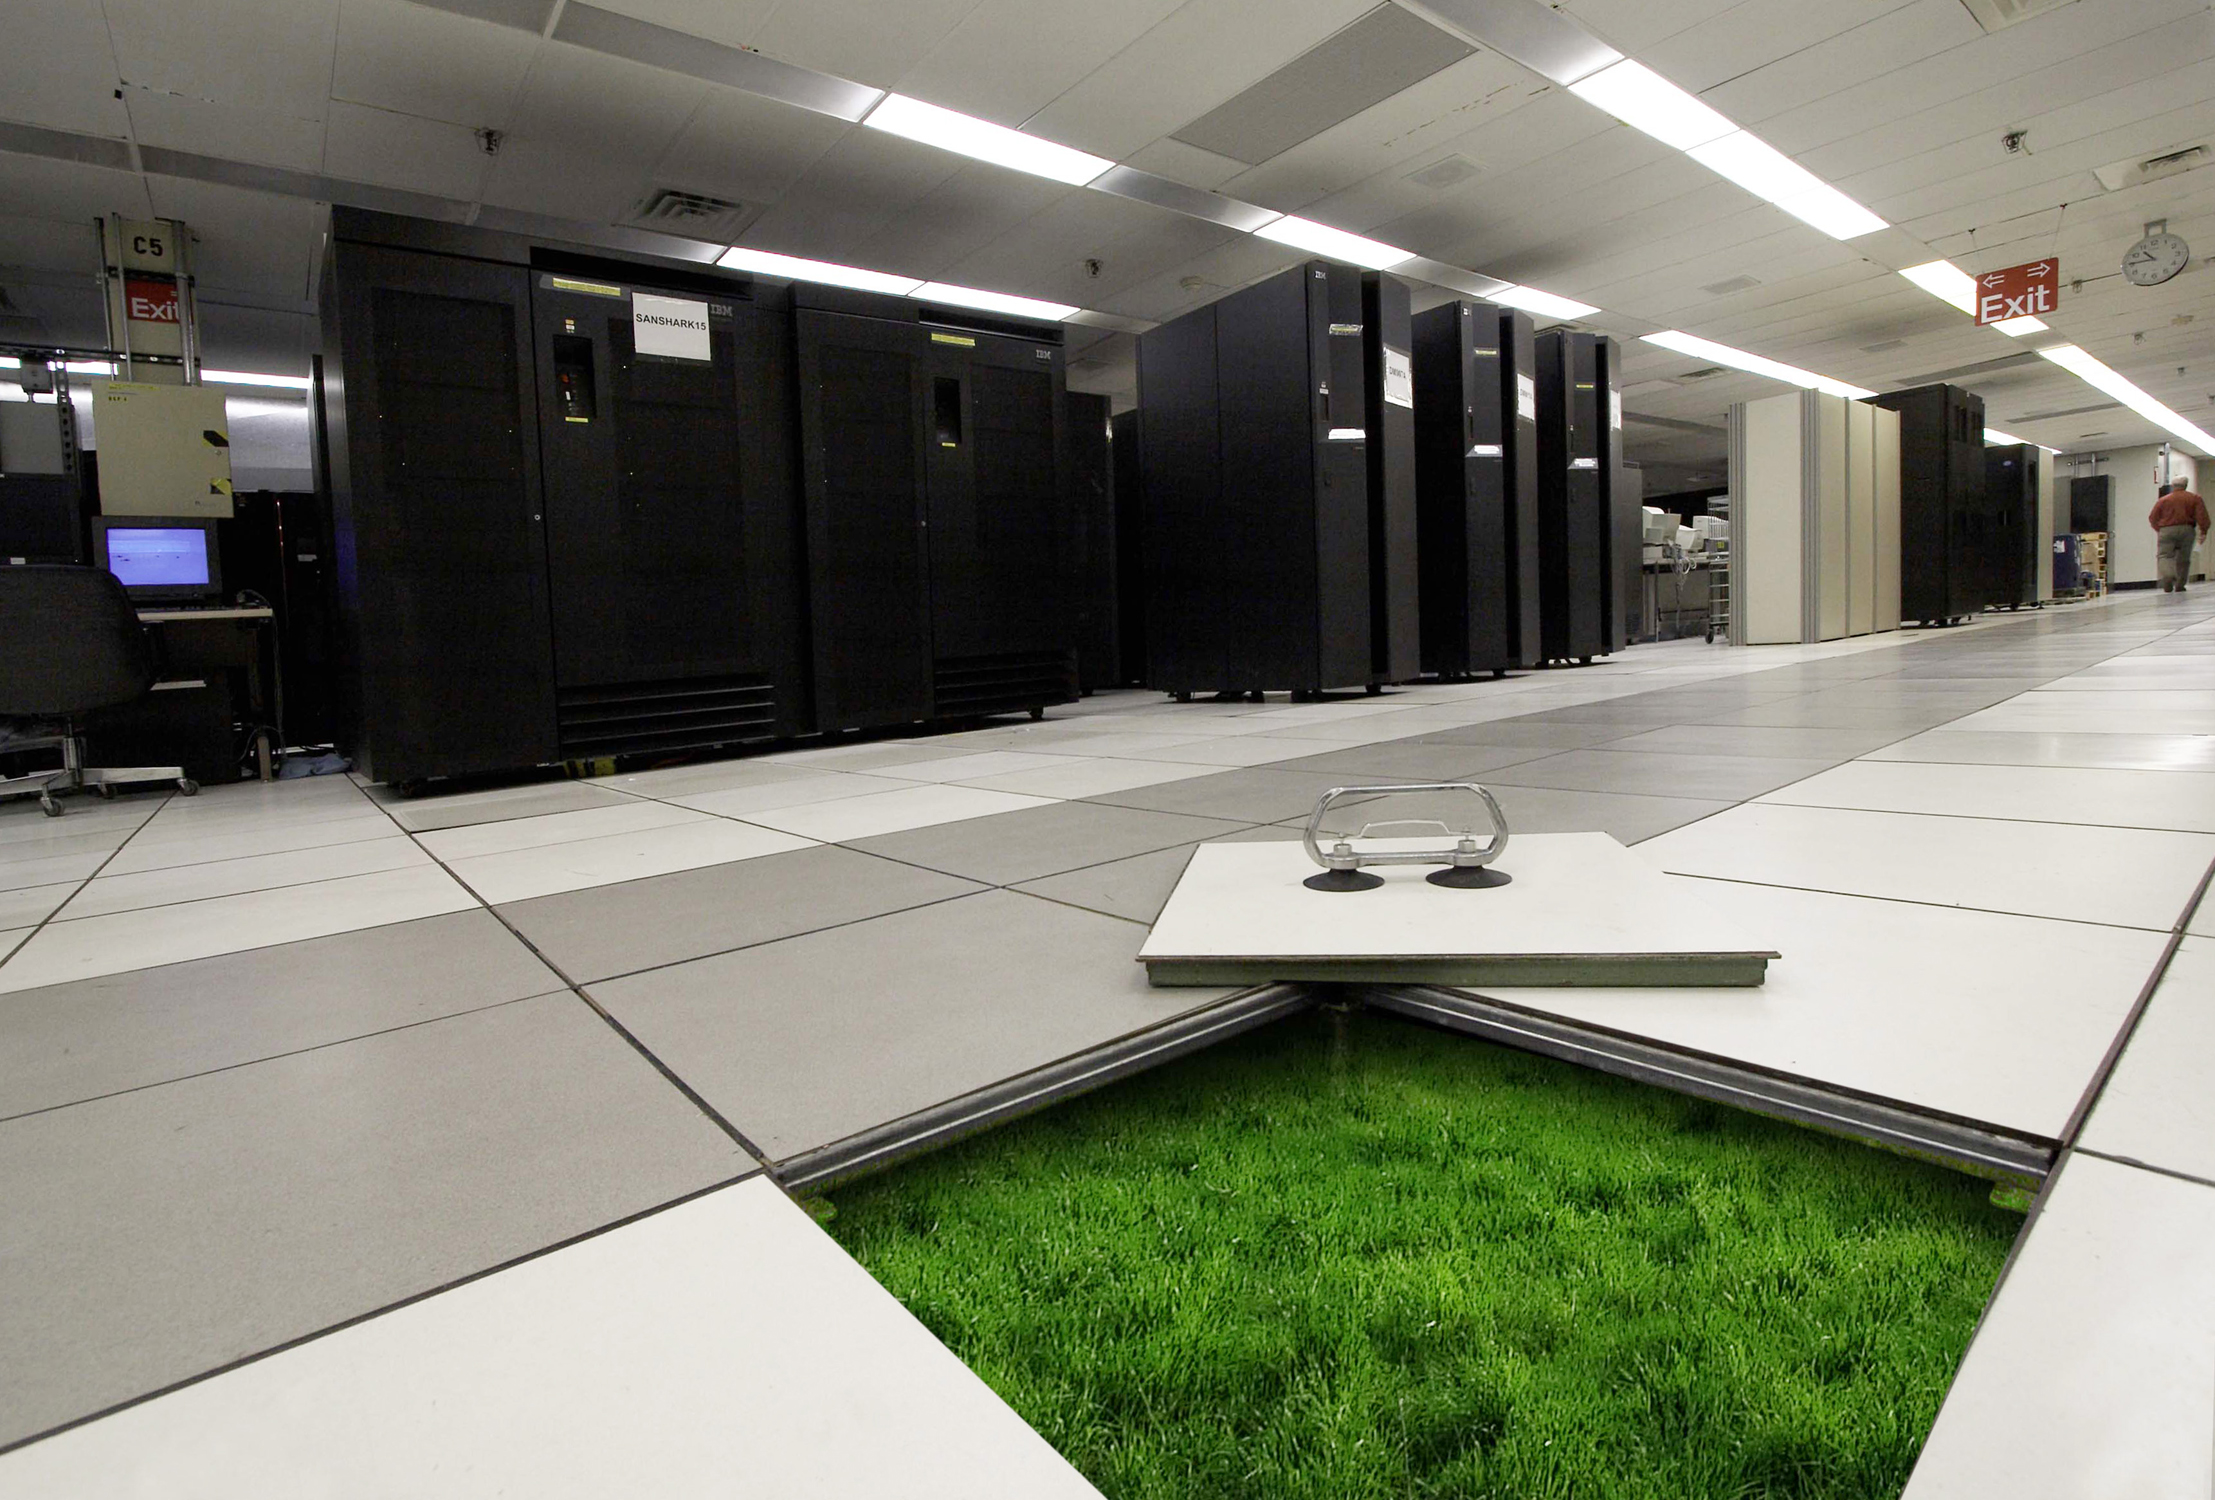
\includegraphics[width=\textwidth]{fig3}
	}
	\caption{Exemplo de figura inserida em uma página A3 no formato horizontal}
	\label{fig5}
\end{figure}

%Retornar ao formato A4
\clearpage
\KOMAoptions{paper=a4, paper=portrait, DIV=15}
\recalctypearea
%-- reinicio em A4 


\subsubsection{Resumo gráfico}

Você pode optar por fazer um resumo no formato de mapa mental/conceitual. 
Aqui foi utilizado o site https://app.mindmup.com para gerar o mapa.

Para utilizar o resumo gráfico, remova o texto da seção resumo (linha 137) e inclua o código para inserir a figura, conforme figura \ref{fig6}

\begin{figure}[h]
	\centering
	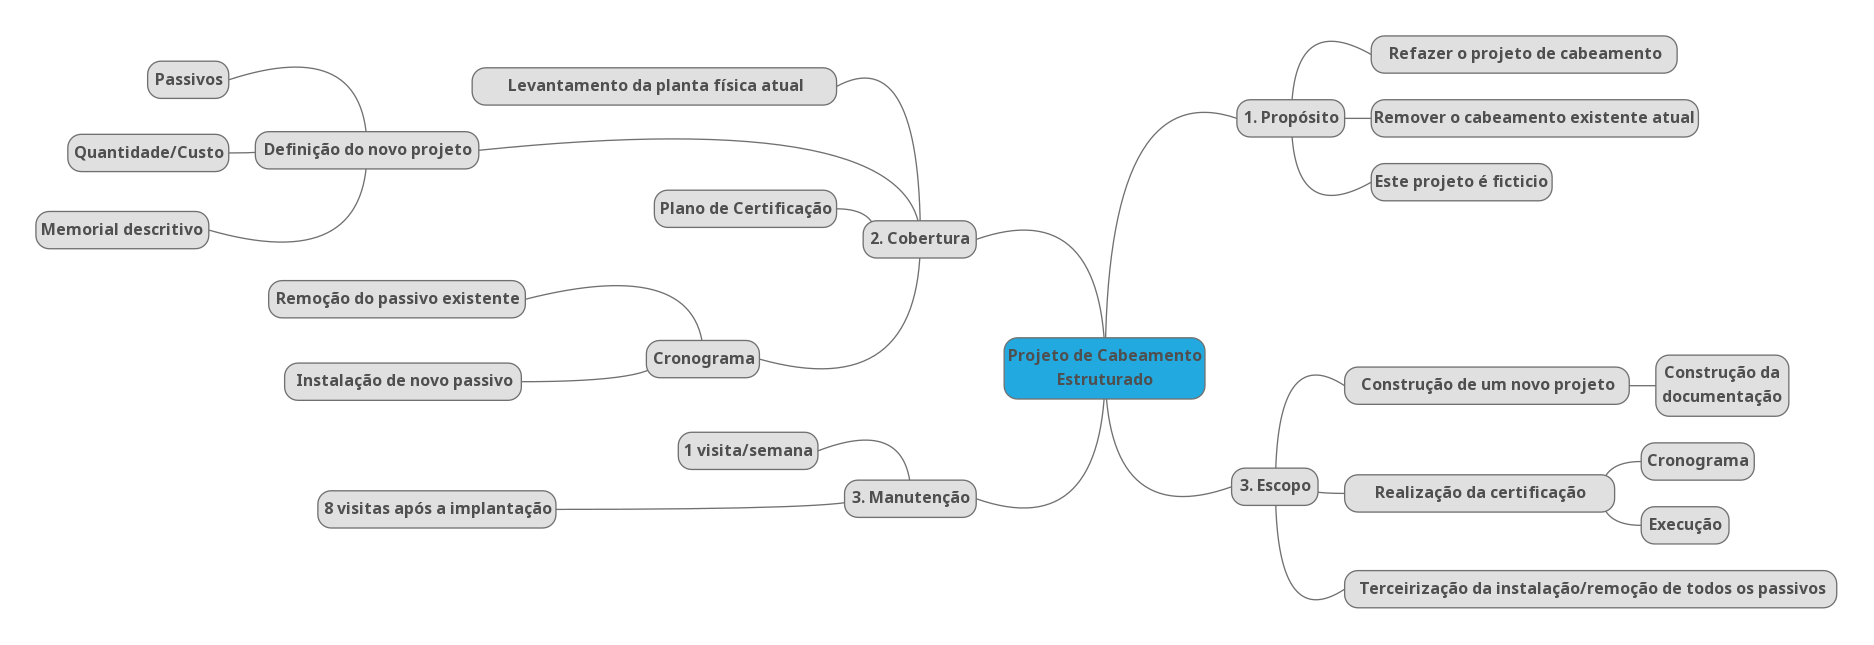
\includegraphics[width=\textwidth,height=5cm,keepaspectratio]{fig4}
	\caption{Exemplo de resumo gráfico}
	\label{fig6}	
\end{figure}

%% ***********************************************************************
%% === ate aqui    =====  ================================================
%% ***********************************************************************

\end{document}